\subsection{XRF Implementation}

\subsubsection{X-ray source}
To incite fluorescence in heavy elements, a high energetic source is needed, as high energy photons is needed to knock their electron out of their orbit. To achieve this a x-ray tube with an Ag anode with an output spectrum as seen in figure \ref{fig:AgSpectra} is recommended. The high energy of the peaks enable the source to achieve fluorescence from elements up to Ag (Z=47), with lesser efficiency up to Sm (Z=62, 40keV).

\begin{figure}[h]
	\centering
	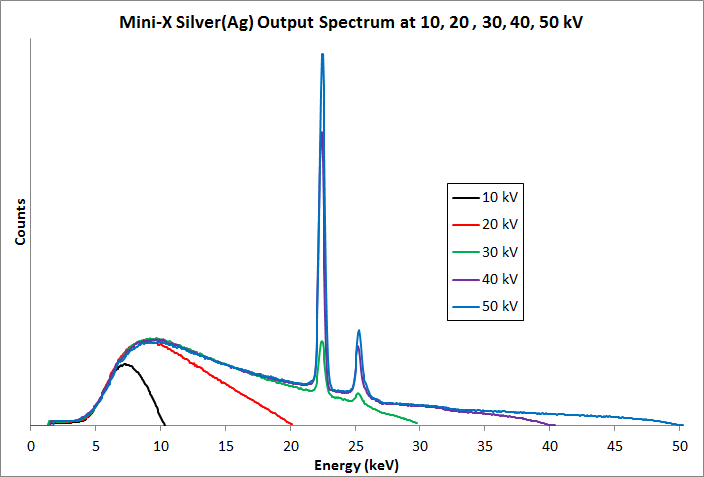
\includegraphics[width=\textwidth]{figures/XRF/minix50_ag6.png}
	\caption{Output spectrum for a x-ray tube using an Ag anode at different voltages.\citep{AmptekSource}}
	\label{fig:AgSpectra}
\end{figure}

The lower end of the energy spectrum is caused by bremsstrahlung in the anode, and is not of much use as it provides little additional resulting fluorescence. The low end is also scattered and will provide a significant noise source for the lower energies. This is particularly undesirable as the lighter elements low energy fluorescence, are also heavily attenuated by the water they are dissolved in. To adjust the spectrum an Al filter can be used to attenuate the lower energies, as seen in figure \ref{fig:AgSpectraFilt}.

\begin{figure}[h]
	\centering
	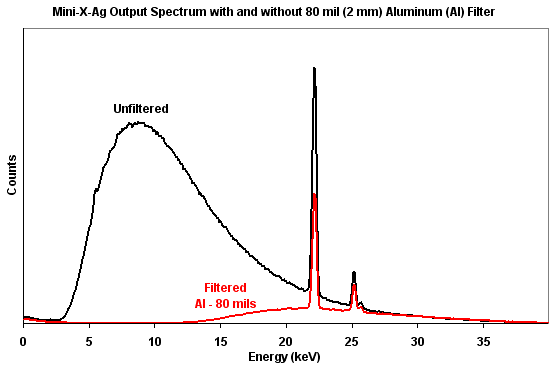
\includegraphics[width=\textwidth]{figures/XRF/minix_Fil.png}
	\caption{Filtered and unfiltered Ag x-ray tube spectrum at 40keV. \citep{AmptekSource}}
	\label{fig:AgSpectraFilt}
\end{figure}


The output spectrum of the x-ray tube have to significant peaks at ~23keV and ~25keV. This is the characteristic lines of Ag when subjected to electron radiation. Knowing these line enables us to take them into account as they will show up as noise in measurements. Focusing on the remaining peaks, and using equation \ref{eq:ComtonEQ}, the Compton scattering resulting from the incident spectrum can be estimated in figure \ref{fig:AgSpectraCompton}.

\begin{figure}[h]
	\centering
	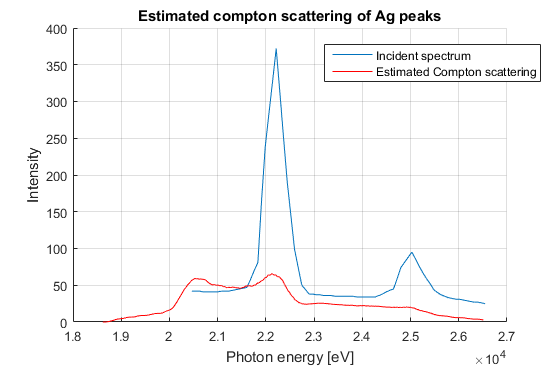
\includegraphics[width=\textwidth]{figures/XRF/estComptonAgPeaks.png}
	\caption{Estimated Compton scattering of the source spectrum.}
	\label{fig:AgSpectraCompton}
\end{figure}

The resulting noise peaks from Compton scattering lies between 20keV and 22.5keV. These will overlap with the $K_\alpha$ of Pd (Z=46, $K_\alpha$ at 21.1keV) and Ag (Z=47, $K_\alpha$ at 22.1keV).

\paragraph{Instrument}
Creating the high voltage needed for the instrument a voltage tripler can be used. The entire instrument can be realized (including high voltage powersupply) with\citep{AmptekSource}:\\
Mass: 360g\\
power: 9W (at max output intensity)\\
Volume: 272.24cm3

\subsubsection{X-ray detector}
When considering the detector the range of encountered photons should be considered. The lighter elements $K_\alpha$ lines are only a few hundred keV apart, to differentiate these a suitable resolution is needed. Detectors also do not perform equally across all energies. The lower limit of the detector is determined by the detector window, as low energy photons are quickly attenuated. The higher limit is determined by the detector material. If we used a polycapillary lens, a window of 25um Be can be used. The detector material can be chosen as Si, as it provides a greater range than what we expect to achieve fluorescence from. In figure \ref{fig:AmptekDetector} a plot of differing detector can be observed. The resolution of the 25um Be SI-PIN detector is sufficient to distinguish elements heavier than Na.

\begin{figure}[h]
	\centering
	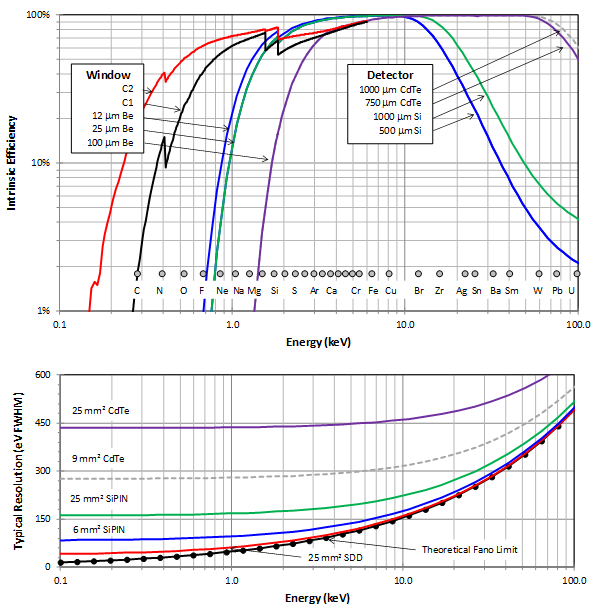
\includegraphics[width=\textwidth]{figures/XRF/EnergyRes.png}
	\caption{\cite{AmptekDetector}}
	\label{fig:AmptekDetector}
\end{figure}





\paragraph{Instrument}
The entire instrument, including high voltage power supply and MCA, can be realized with\citep{AmptekDetector}:\\
Mass: 180g\\
power: 4W max, 2.5W typical\\
Volume: 175cm3



\subsubsection{Mass, power and volume}




